% Options for packages loaded elsewhere
\PassOptionsToPackage{unicode}{hyperref}
\PassOptionsToPackage{hyphens}{url}
%
\documentclass[
]{article}
\usepackage{amsmath,amssymb}
\usepackage{iftex}
\ifPDFTeX
  \usepackage[T1]{fontenc}
  \usepackage[utf8]{inputenc}
  \usepackage{textcomp} % provide euro and other symbols
\else % if luatex or xetex
  \usepackage{unicode-math} % this also loads fontspec
  \defaultfontfeatures{Scale=MatchLowercase}
  \defaultfontfeatures[\rmfamily]{Ligatures=TeX,Scale=1}
\fi
\usepackage{lmodern}
\ifPDFTeX\else
  % xetex/luatex font selection
\fi
% Use upquote if available, for straight quotes in verbatim environments
\IfFileExists{upquote.sty}{\usepackage{upquote}}{}
\IfFileExists{microtype.sty}{% use microtype if available
  \usepackage[]{microtype}
  \UseMicrotypeSet[protrusion]{basicmath} % disable protrusion for tt fonts
}{}
\makeatletter
\@ifundefined{KOMAClassName}{% if non-KOMA class
  \IfFileExists{parskip.sty}{%
    \usepackage{parskip}
  }{% else
    \setlength{\parindent}{0pt}
    \setlength{\parskip}{6pt plus 2pt minus 1pt}}
}{% if KOMA class
  \KOMAoptions{parskip=half}}
\makeatother
\usepackage{xcolor}
\usepackage[margin=1in]{geometry}
\usepackage{color}
\usepackage{fancyvrb}
\newcommand{\VerbBar}{|}
\newcommand{\VERB}{\Verb[commandchars=\\\{\}]}
\DefineVerbatimEnvironment{Highlighting}{Verbatim}{commandchars=\\\{\}}
% Add ',fontsize=\small' for more characters per line
\usepackage{framed}
\definecolor{shadecolor}{RGB}{248,248,248}
\newenvironment{Shaded}{\begin{snugshade}}{\end{snugshade}}
\newcommand{\AlertTok}[1]{\textcolor[rgb]{0.94,0.16,0.16}{#1}}
\newcommand{\AnnotationTok}[1]{\textcolor[rgb]{0.56,0.35,0.01}{\textbf{\textit{#1}}}}
\newcommand{\AttributeTok}[1]{\textcolor[rgb]{0.13,0.29,0.53}{#1}}
\newcommand{\BaseNTok}[1]{\textcolor[rgb]{0.00,0.00,0.81}{#1}}
\newcommand{\BuiltInTok}[1]{#1}
\newcommand{\CharTok}[1]{\textcolor[rgb]{0.31,0.60,0.02}{#1}}
\newcommand{\CommentTok}[1]{\textcolor[rgb]{0.56,0.35,0.01}{\textit{#1}}}
\newcommand{\CommentVarTok}[1]{\textcolor[rgb]{0.56,0.35,0.01}{\textbf{\textit{#1}}}}
\newcommand{\ConstantTok}[1]{\textcolor[rgb]{0.56,0.35,0.01}{#1}}
\newcommand{\ControlFlowTok}[1]{\textcolor[rgb]{0.13,0.29,0.53}{\textbf{#1}}}
\newcommand{\DataTypeTok}[1]{\textcolor[rgb]{0.13,0.29,0.53}{#1}}
\newcommand{\DecValTok}[1]{\textcolor[rgb]{0.00,0.00,0.81}{#1}}
\newcommand{\DocumentationTok}[1]{\textcolor[rgb]{0.56,0.35,0.01}{\textbf{\textit{#1}}}}
\newcommand{\ErrorTok}[1]{\textcolor[rgb]{0.64,0.00,0.00}{\textbf{#1}}}
\newcommand{\ExtensionTok}[1]{#1}
\newcommand{\FloatTok}[1]{\textcolor[rgb]{0.00,0.00,0.81}{#1}}
\newcommand{\FunctionTok}[1]{\textcolor[rgb]{0.13,0.29,0.53}{\textbf{#1}}}
\newcommand{\ImportTok}[1]{#1}
\newcommand{\InformationTok}[1]{\textcolor[rgb]{0.56,0.35,0.01}{\textbf{\textit{#1}}}}
\newcommand{\KeywordTok}[1]{\textcolor[rgb]{0.13,0.29,0.53}{\textbf{#1}}}
\newcommand{\NormalTok}[1]{#1}
\newcommand{\OperatorTok}[1]{\textcolor[rgb]{0.81,0.36,0.00}{\textbf{#1}}}
\newcommand{\OtherTok}[1]{\textcolor[rgb]{0.56,0.35,0.01}{#1}}
\newcommand{\PreprocessorTok}[1]{\textcolor[rgb]{0.56,0.35,0.01}{\textit{#1}}}
\newcommand{\RegionMarkerTok}[1]{#1}
\newcommand{\SpecialCharTok}[1]{\textcolor[rgb]{0.81,0.36,0.00}{\textbf{#1}}}
\newcommand{\SpecialStringTok}[1]{\textcolor[rgb]{0.31,0.60,0.02}{#1}}
\newcommand{\StringTok}[1]{\textcolor[rgb]{0.31,0.60,0.02}{#1}}
\newcommand{\VariableTok}[1]{\textcolor[rgb]{0.00,0.00,0.00}{#1}}
\newcommand{\VerbatimStringTok}[1]{\textcolor[rgb]{0.31,0.60,0.02}{#1}}
\newcommand{\WarningTok}[1]{\textcolor[rgb]{0.56,0.35,0.01}{\textbf{\textit{#1}}}}
\usepackage{graphicx}
\makeatletter
\def\maxwidth{\ifdim\Gin@nat@width>\linewidth\linewidth\else\Gin@nat@width\fi}
\def\maxheight{\ifdim\Gin@nat@height>\textheight\textheight\else\Gin@nat@height\fi}
\makeatother
% Scale images if necessary, so that they will not overflow the page
% margins by default, and it is still possible to overwrite the defaults
% using explicit options in \includegraphics[width, height, ...]{}
\setkeys{Gin}{width=\maxwidth,height=\maxheight,keepaspectratio}
% Set default figure placement to htbp
\makeatletter
\def\fps@figure{htbp}
\makeatother
\setlength{\emergencystretch}{3em} % prevent overfull lines
\providecommand{\tightlist}{%
  \setlength{\itemsep}{0pt}\setlength{\parskip}{0pt}}
\setcounter{secnumdepth}{-\maxdimen} % remove section numbering
\ifLuaTeX
  \usepackage{selnolig}  % disable illegal ligatures
\fi
\IfFileExists{bookmark.sty}{\usepackage{bookmark}}{\usepackage{hyperref}}
\IfFileExists{xurl.sty}{\usepackage{xurl}}{} % add URL line breaks if available
\urlstyle{same}
\hypersetup{
  pdftitle={A cheat sheet to `tidy' data processing for ECOL 4000/6000},
  pdfauthor={Katie Schroeder (k.schroeder@uga.edu)},
  hidelinks,
  pdfcreator={LaTeX via pandoc}}

\title{A cheat sheet to `tidy' data processing for ECOL 4000/6000}
\author{Katie Schroeder
(\href{mailto:k.schroeder@uga.edu}{\nolinkurl{k.schroeder@uga.edu}})}
\date{2023-10-13}

\begin{document}
\maketitle

\hypertarget{topic-1-basics---setting-your-working-directory-install-and-calling-packages}{%
\paragraph{Topic 1: Basics - setting your working directory, install and
calling
packages}\label{topic-1-basics---setting-your-working-directory-install-and-calling-packages}}

\textbf{Setting your working directory:}\\
This step is really important and tells R where you're grabbing files
from on your computer. There are a couple options for setting your
working directory:

\begin{itemize}
\tightlist
\item
  set it manually using the \texttt{setwd()} command

  \begin{itemize}
  \tightlist
  \item
    Ex: setwd(``\textasciitilde/User/Dawg1/Documents'')\\
  \end{itemize}
\item
  set it to the source file location

  \begin{itemize}
  \tightlist
  \item
    If your script is saved in the same location as the files you will
    be loading, you can go to the session menu, select ``Set working
    directory'' and then select ``To source file location''
  \end{itemize}
\item
  set it to a folder you browse for

  \begin{itemize}
  \tightlist
  \item
    You can select your working directory location by going to the
    session menu, selecting ``Set working directory'' and then selecting
    ``Choose directory''
  \end{itemize}
\end{itemize}

\textbf{Installing a package:}\\
We've used a few packages in this class so far (one example is
tidyverse). As you work more with R, you may find more and more useful
packages. If you don't have a package on your computer, you'll have to
install it using \texttt{install.packages()}. Make sure you put the name
of the package in quotes when you're using \texttt{install.packages()}

\textbf{Calling a package from your library:}\\
If you have a package installed, it's in your library, but will not be
automatically loaded when you start a new R session. To use the
functions in that package, you'll need to call it from your library.\\
For example, if we want to use \texttt{ggplot()}, we'll need to call
tidyverse using the \texttt{library()} command.\\
Example: \texttt{library(tidyverse)}

Side note: You could also use library(ggplot2) if you were just using
ggplot functions. tidyverse is a bit of a super package that contains a
lot of other packages (including ggplot2).

\hypertarget{topic-2-reading-in-data-and-viewing-it}{%
\paragraph{Topic 2: Reading in data and viewing
it}\label{topic-2-reading-in-data-and-viewing-it}}

Often times we'll read things in as .csv files using \texttt{read.csv}

For the bears problem set, we used the following code:

\begin{Shaded}
\begin{Highlighting}[]
\NormalTok{bears}\OtherTok{\textless{}{-}} \FunctionTok{read.csv}\NormalTok{(}\StringTok{"PS1\_Data\_Bears.csv"}\NormalTok{)}
\end{Highlighting}
\end{Shaded}

\textbf{Viewing the data frame:}

To view the bears data frame, there are a couple options:

\begin{itemize}
\tightlist
\item
  You can type \texttt{View(bears)} into the console or into your
  script\\
\item
  You can click on bears in the global environment
\end{itemize}

Some options for looking at your data:

\begin{itemize}
\tightlist
\item
  Overview of the entire data frame:

  \begin{itemize}
  \tightlist
  \item
    \texttt{str()} gives an overview of the length, column names, and
    the type of data (number, character, integer, etc.) in each column\\
  \item
    \texttt{head()} gives the first six rows of your data frame\\
  \item
    \texttt{summary()} gives a summary of each column in your data frame
    (quantiles, minimums, maximums)\\
  \end{itemize}
\item
  For specific columns - remember to use the \$ operator to specify the
  column!

  \begin{itemize}
  \tightlist
  \item
    \texttt{sum()} the total in a column\\
  \item
    \texttt{min()} \texttt{mean()} \texttt{median()} and \texttt{max()}
    for those summary stats
  \end{itemize}
\end{itemize}

\textbf{Subsetting the data frame:}

The brackets method from the bears problem set:

\begin{Shaded}
\begin{Highlighting}[]
\CommentTok{\#getting a single column, females}
\NormalTok{bears[,}\DecValTok{2}\NormalTok{] }\CommentTok{\#second column}
\NormalTok{bears}\SpecialCharTok{$}\NormalTok{females }\CommentTok{\#equivalent }

\CommentTok{\#making two data frames for data before and after 1976}
\NormalTok{bears1 }\OtherTok{\textless{}{-}}\NormalTok{ bears[bears}\SpecialCharTok{$}\NormalTok{year}\SpecialCharTok{\textless{}}\DecValTok{1977}\NormalTok{,]}
\NormalTok{bears2 }\OtherTok{\textless{}{-}}\NormalTok{ bears[bears}\SpecialCharTok{$}\NormalTok{year}\SpecialCharTok{\textgreater{}}\DecValTok{1975}\NormalTok{,]}
\end{Highlighting}
\end{Shaded}

Tidyverse options:

\begin{Shaded}
\begin{Highlighting}[]
\CommentTok{\#load tidyverse}
\FunctionTok{library}\NormalTok{(tidyverse)}

\CommentTok{\#getting a single column}
\NormalTok{bears }\SpecialCharTok{\%\textgreater{}\%} \FunctionTok{select}\NormalTok{(females)}

\CommentTok{\#subsetting before and after 1976}
\NormalTok{bears1 }\OtherTok{\textless{}{-}}\NormalTok{ bears }\SpecialCharTok{\%\textgreater{}\%} \FunctionTok{filter}\NormalTok{(year}\SpecialCharTok{\textless{}}\DecValTok{1977}\NormalTok{)}
\NormalTok{bears2 }\OtherTok{\textless{}{-}}\NormalTok{ bears }\SpecialCharTok{\%\textgreater{}\%} \FunctionTok{filter}\NormalTok{(year}\SpecialCharTok{\textgreater{}}\DecValTok{1975}\NormalTok{)}
\end{Highlighting}
\end{Shaded}

\hypertarget{topic-3-plotting}{%
\paragraph{Topic 3: Plotting}\label{topic-3-plotting}}

Example from the bears problem set:

\begin{Shaded}
\begin{Highlighting}[]
\FunctionTok{plot}\NormalTok{(bears}\SpecialCharTok{$}\NormalTok{year,}
\NormalTok{     bears}\SpecialCharTok{$}\NormalTok{females,}
     \AttributeTok{xlab=}\StringTok{"Year"}\NormalTok{,}
     \AttributeTok{ylab=}\StringTok{"Number of females"}\NormalTok{, }
     \AttributeTok{col=}\StringTok{"forestgreen"}\NormalTok{, }
     \AttributeTok{type=}\StringTok{"o"}\NormalTok{, }
     \AttributeTok{pch=}\DecValTok{20}\NormalTok{)}
\end{Highlighting}
\end{Shaded}

\includegraphics{tidy_cheatsheet_for_group_project_files/figure-latex/unnamed-chunk-4-1.pdf}

\begin{Shaded}
\begin{Highlighting}[]
\CommentTok{\# a tidyverse option: }
\FunctionTok{ggplot}\NormalTok{(bears,}\FunctionTok{aes}\NormalTok{(}\AttributeTok{x=}\NormalTok{year,}\AttributeTok{y=}\NormalTok{females)) }\SpecialCharTok{+}
  \FunctionTok{geom\_point}\NormalTok{() }\SpecialCharTok{+}
  \FunctionTok{geom\_line}\NormalTok{() }\SpecialCharTok{+}
  \FunctionTok{xlab}\NormalTok{(}\StringTok{"Year"}\NormalTok{) }\SpecialCharTok{+}
  \FunctionTok{ylab}\NormalTok{(}\StringTok{"Number of females"}\NormalTok{) }\SpecialCharTok{+}
  \FunctionTok{theme\_classic}\NormalTok{()}
\end{Highlighting}
\end{Shaded}

\includegraphics{tidy_cheatsheet_for_group_project_files/figure-latex/unnamed-chunk-4-2.pdf}

\textbf{Commands for more advanced plotting in ggplot}

ggplot cheat sheet page 1: 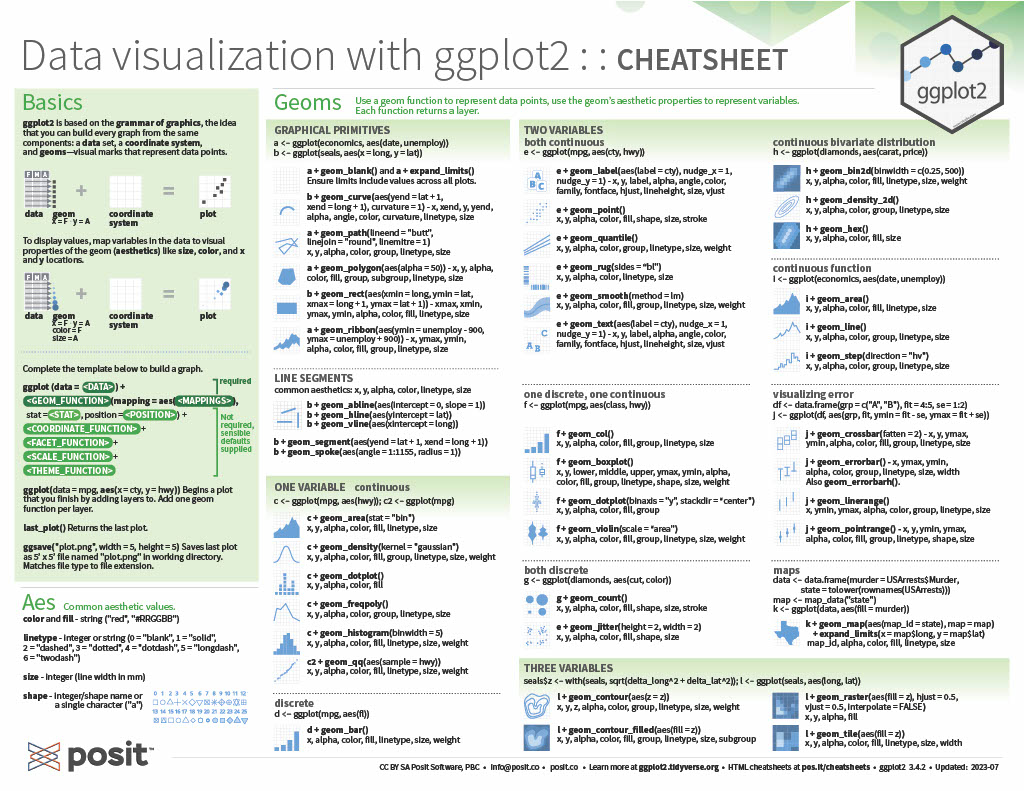
\includegraphics{page1.jpg}

ggplot cheat sheet page 2: 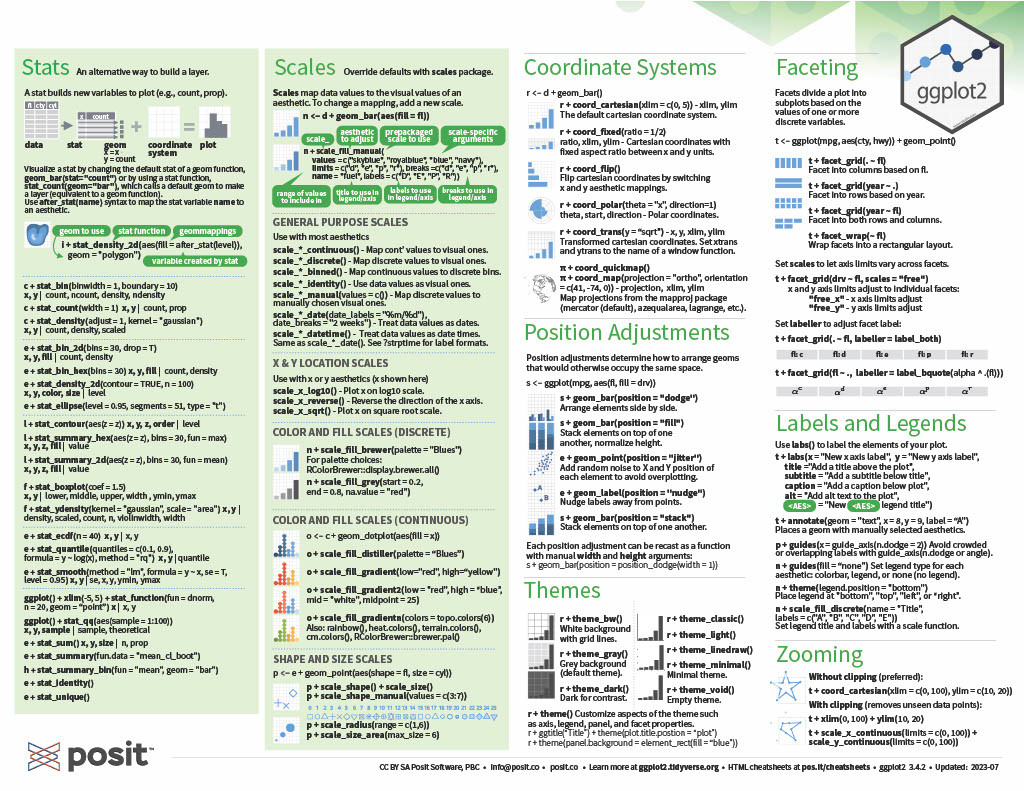
\includegraphics{page2.jpg}

\hypertarget{topic-4-calculating-different-response-variables}{%
\paragraph{Topic 4: Calculating different response
variables}\label{topic-4-calculating-different-response-variables}}

In problem set 2, we calculated lambda for the terns on all of the
islands using a for loop:

\begin{Shaded}
\begin{Highlighting}[]
\NormalTok{terns }\OtherTok{\textless{}{-}} \FunctionTok{read.csv}\NormalTok{(}\StringTok{"PS2\_data\_terns.csv"}\NormalTok{)}

\CommentTok{\#calculate the total terns by adding together the terns from each island}
\NormalTok{terns}\SpecialCharTok{$}\NormalTok{total }\OtherTok{\textless{}{-}}\NormalTok{ terns}\SpecialCharTok{$}\NormalTok{bird }\SpecialCharTok{+}\NormalTok{ terns}\SpecialCharTok{$}\NormalTok{ram }\SpecialCharTok{+}\NormalTok{ terns}\SpecialCharTok{$}\NormalTok{pikense}

\CommentTok{\#create an empty column for the growth rate to populate}
\NormalTok{terns}\SpecialCharTok{$}\NormalTok{total\_growth\_rate }\OtherTok{\textless{}{-}} \ConstantTok{NA}

\ControlFlowTok{for}\NormalTok{(i }\ControlFlowTok{in} \DecValTok{2}\SpecialCharTok{:}\FunctionTok{length}\NormalTok{(terns}\SpecialCharTok{$}\NormalTok{year))\{ }\CommentTok{\# initiate the loop with "for"}
\NormalTok{  terns}\SpecialCharTok{$}\NormalTok{total\_growth\_rate[i] }\OtherTok{\textless{}{-}}\NormalTok{ terns}\SpecialCharTok{$}\NormalTok{total[i]}\SpecialCharTok{/}\NormalTok{terns}\SpecialCharTok{$}\NormalTok{total[i}\DecValTok{{-}1}\NormalTok{] }
  \CommentTok{\# calculate the growth rate as the ratio between population size now and population size one year ago}
\NormalTok{  \} }\CommentTok{\# close the loop}
\end{Highlighting}
\end{Shaded}

We could have also done this calculation using the \texttt{lag()}
command in the package \texttt{dplyr}. \texttt{dplyr} is another package
in tidyverse. \texttt{lag()} can be used to create column that is one
row behind the column we input.

\begin{Shaded}
\begin{Highlighting}[]
\NormalTok{terns}\SpecialCharTok{$}\NormalTok{total\_N0 }\OtherTok{\textless{}{-}} \FunctionTok{lag}\NormalTok{(terns}\SpecialCharTok{$}\NormalTok{total) }\CommentTok{\#lag function makes a new column with total column shifted down a row (lag=1)}

\CommentTok{\#calculate lambda by dividing total at N+1 by total at N}
\NormalTok{terns}\SpecialCharTok{$}\NormalTok{lambda }\OtherTok{\textless{}{-}}\NormalTok{ terns}\SpecialCharTok{$}\NormalTok{total }\SpecialCharTok{/}\NormalTok{ terns}\SpecialCharTok{$}\NormalTok{total\_N0}
\end{Highlighting}
\end{Shaded}

If we compare the two lambas we calculated, total\_growth rate using a
loop and lambda using lag, we can see they lead to the same result:

\begin{Shaded}
\begin{Highlighting}[]
\FunctionTok{ggplot}\NormalTok{(terns,}\FunctionTok{aes}\NormalTok{(}\AttributeTok{x=}\NormalTok{total,}\AttributeTok{y=}\NormalTok{total\_growth\_rate)) }\SpecialCharTok{+}
  \FunctionTok{geom\_point}\NormalTok{() }\SpecialCharTok{+} \FunctionTok{theme\_classic}\NormalTok{()}
\end{Highlighting}
\end{Shaded}

\includegraphics{tidy_cheatsheet_for_group_project_files/figure-latex/unnamed-chunk-7-1.pdf}

\begin{Shaded}
\begin{Highlighting}[]
\FunctionTok{ggplot}\NormalTok{(terns,}\FunctionTok{aes}\NormalTok{(}\AttributeTok{x=}\NormalTok{total,}\AttributeTok{y=}\NormalTok{lambda)) }\SpecialCharTok{+}
  \FunctionTok{geom\_point}\NormalTok{() }\SpecialCharTok{+}\FunctionTok{theme\_classic}\NormalTok{()}
\end{Highlighting}
\end{Shaded}

\includegraphics{tidy_cheatsheet_for_group_project_files/figure-latex/unnamed-chunk-7-2.pdf}

In the tern example, we also fit a line to these data. In base r, we
used \texttt{abline()} and \texttt{lm()} (linear model). We can do the
same in ggplot using \texttt{geom\_smooth()}

\begin{Shaded}
\begin{Highlighting}[]
\CommentTok{\#base r}
\FunctionTok{plot}\NormalTok{(terns}\SpecialCharTok{$}\NormalTok{total, terns}\SpecialCharTok{$}\NormalTok{total\_growth\_rate)}
\FunctionTok{abline}\NormalTok{(}\FunctionTok{lm}\NormalTok{(total\_growth\_rate}\SpecialCharTok{\textasciitilde{}}\NormalTok{total, }\AttributeTok{data=}\NormalTok{terns))}
\end{Highlighting}
\end{Shaded}

\includegraphics{tidy_cheatsheet_for_group_project_files/figure-latex/unnamed-chunk-8-1.pdf}

\begin{Shaded}
\begin{Highlighting}[]
\CommentTok{\#tidyverse option}
\FunctionTok{ggplot}\NormalTok{(terns,}\FunctionTok{aes}\NormalTok{(}\AttributeTok{x=}\NormalTok{total,}\AttributeTok{y=}\NormalTok{lambda)) }\SpecialCharTok{+}
  \FunctionTok{geom\_point}\NormalTok{() }\SpecialCharTok{+}
  \FunctionTok{geom\_smooth}\NormalTok{(}\AttributeTok{method=}\StringTok{\textquotesingle{}lm\textquotesingle{}}\NormalTok{,}\AttributeTok{se=}\NormalTok{F) }\SpecialCharTok{+} \CommentTok{\#se=F here means it will just show the line and not an estimate of the error associated with the fit}
  \FunctionTok{theme\_classic}\NormalTok{()}
\end{Highlighting}
\end{Shaded}

\begin{verbatim}
## `geom_smooth()` using formula = 'y ~ x'
\end{verbatim}

\includegraphics{tidy_cheatsheet_for_group_project_files/figure-latex/unnamed-chunk-8-2.pdf}

\hypertarget{topic-5-working-with-the-srs-zooplankton-data}{%
\paragraph{Topic 5: Working with the SRS zooplankton
data}\label{topic-5-working-with-the-srs-zooplankton-data}}

We often want to know how many of a certain thing we have. For one of
the problem sets, we calculated the number of unique taxa using
\texttt{length()} and \texttt{unique()}

\begin{Shaded}
\begin{Highlighting}[]
\NormalTok{zoop }\OtherTok{\textless{}{-}} \FunctionTok{read.csv}\NormalTok{(}\StringTok{"SRS\_zoop.csv"}\NormalTok{)}
\CommentTok{\#number of different taxa }
\FunctionTok{length}\NormalTok{(}\FunctionTok{unique}\NormalTok{(zoop}\SpecialCharTok{$}\NormalTok{taxa))}
\end{Highlighting}
\end{Shaded}

\begin{verbatim}
## [1] 133
\end{verbatim}

\begin{Shaded}
\begin{Highlighting}[]
\CommentTok{\#number of bays}
\FunctionTok{length}\NormalTok{(}\FunctionTok{unique}\NormalTok{(zoop}\SpecialCharTok{$}\NormalTok{bay))}
\end{Highlighting}
\end{Shaded}

\begin{verbatim}
## [1] 14
\end{verbatim}

From this, we see that there are 133 different taxa found in the 14
different bays.

We may want to ask about unique taxa in each bay. We could subset and
create data frames for each of the bays like we did for the bears data
or we could create a loop, but we can also use tidyverse syntax and the
\texttt{group\_by()} and \texttt{summarize()} commands. Within
summarize, we're using \texttt{n\_distinct()} which counts the number of
distinct observations in the specified column.

\begin{Shaded}
\begin{Highlighting}[]
\NormalTok{zoop }\SpecialCharTok{\%\textgreater{}\%} \FunctionTok{group\_by}\NormalTok{(bay) }\SpecialCharTok{\%\textgreater{}\%}
  \FunctionTok{summarize}\NormalTok{(}\AttributeTok{unique\_taxa =} \FunctionTok{n\_distinct}\NormalTok{(taxa))}
\end{Highlighting}
\end{Shaded}

\begin{verbatim}
## # A tibble: 14 x 2
##      bay unique_taxa
##    <int>       <int>
##  1     3          72
##  2     4          54
##  3     7          59
##  4     9          59
##  5    11          70
##  6    25          52
##  7    26          71
##  8    40          71
##  9    41          62
## 10    44          54
## 11    66          60
## 12    78          93
## 13    79          35
## 14    80          37
\end{verbatim}

\textbf{Other loop and tidyverse equivalent processes from working with
these data in the problem sets:}

In the problem set, we calculated abundance of each of the taxa using
this code:

\begin{Shaded}
\begin{Highlighting}[]
\NormalTok{taxa }\OtherTok{\textless{}{-}} \FunctionTok{unique}\NormalTok{(zoop}\SpecialCharTok{$}\NormalTok{taxa) }\CommentTok{\# first step is to create a list of all taxa}
\NormalTok{total.abundance }\OtherTok{\textless{}{-}} \FunctionTok{data.frame}\NormalTok{(}\AttributeTok{taxa=}\NormalTok{taxa) }\CommentTok{\# then create an empty dataframe}
\CommentTok{\# that just includes the names of the taxa. then, we\textquotesingle{}ll fill in a second}
\CommentTok{\# column of the dataframe with our loop:}
\ControlFlowTok{for}\NormalTok{(i }\ControlFlowTok{in} \DecValTok{1}\SpecialCharTok{:}\FunctionTok{length}\NormalTok{(taxa))\{}
\NormalTok{  zoop.subset }\OtherTok{\textless{}{-}}\NormalTok{ zoop[zoop}\SpecialCharTok{$}\NormalTok{taxa}\SpecialCharTok{==}\NormalTok{taxa[i],] }\CommentTok{\# subset the data to only include}
  \CommentTok{\# rows where taxa i is observed. }
\NormalTok{  total.abundance}\SpecialCharTok{$}\NormalTok{abundance[i] }\OtherTok{\textless{}{-}} \FunctionTok{sum}\NormalTok{(zoop.subset}\SpecialCharTok{$}\NormalTok{abund, }\AttributeTok{na.rm=}\NormalTok{T)}
  \CommentTok{\# sum up the total abundance of that taxa, after removing NAs}
  \CommentTok{\# and input it as the i\textquotesingle{}ith observation in the summary dataframe}
\NormalTok{\}}

\CommentTok{\#we can use head to see the first six rows of our sorted abundance data frame}
\FunctionTok{head}\NormalTok{(total.abundance[}\FunctionTok{order}\NormalTok{(total.abundance}\SpecialCharTok{$}\NormalTok{abundance),])}
\end{Highlighting}
\end{Shaded}

\begin{verbatim}
##                  taxa abundance
## 15          Alona sp.         1
## 41      Curculionidae         1
## 52      Diptera larva         1
## 54  Dunhevedia crassa         1
## 85        Lepidoptera         1
## 101           Nepidae         1
\end{verbatim}

\begin{Shaded}
\begin{Highlighting}[]
\CommentTok{\#adding a minus sign in front of the column we want to sort using order sorts it the opposite direction (descending)}
\FunctionTok{head}\NormalTok{(total.abundance[}\FunctionTok{order}\NormalTok{(}\SpecialCharTok{{-}}\NormalTok{total.abundance}\SpecialCharTok{$}\NormalTok{abundance),])}
\end{Highlighting}
\end{Shaded}

\begin{verbatim}
##                        taxa abundance
## 42               Cyclopoida    113593
## 21          Bosmina tubicen     59437
## 107               Ostracoda     37760
## 51  Diaphanosoma brachyurum     35520
## 22           Calanoida juv.     31321
## 43           Daphnia laevis     19662
\end{verbatim}

There's also an option to do the same thing in tidyverse. In this
example, we group the data by taxa and then summarize each of those
groups by summing abundance. We can then compare the first and last six
values we get from this method.

\begin{Shaded}
\begin{Highlighting}[]
\NormalTok{total\_abundance}\OtherTok{\textless{}{-}}\NormalTok{zoop }\SpecialCharTok{\%\textgreater{}\%} \FunctionTok{group\_by}\NormalTok{(taxa) }\SpecialCharTok{\%\textgreater{}\%}
  \FunctionTok{summarize}\NormalTok{(}\AttributeTok{abundance=}\FunctionTok{sum}\NormalTok{(abund,}\AttributeTok{na.rm=}\NormalTok{T))}

\CommentTok{\# to sort using pipes, we use arrange and then head to get the first 6 rows of that arrange data}
\NormalTok{total\_abundance }\SpecialCharTok{\%\textgreater{}\%} \FunctionTok{arrange}\NormalTok{(abundance) }\SpecialCharTok{\%\textgreater{}\%} \FunctionTok{head}\NormalTok{()}
\end{Highlighting}
\end{Shaded}

\begin{verbatim}
## # A tibble: 6 x 2
##   taxa              abundance
##   <chr>                 <int>
## 1 Alona sp.                 1
## 2 Curculionidae             1
## 3 Diptera larva             1
## 4 Dunhevedia crassa         1
## 5 Lepidoptera               1
## 6 Nepidae                   1
\end{verbatim}

\begin{Shaded}
\begin{Highlighting}[]
\CommentTok{\# to sort so abundance is descending, we use arrange with desc (for descending)}
\NormalTok{total\_abundance }\SpecialCharTok{\%\textgreater{}\%} \FunctionTok{arrange}\NormalTok{(}\FunctionTok{desc}\NormalTok{(abundance)) }\SpecialCharTok{\%\textgreater{}\%} \FunctionTok{head}\NormalTok{()}
\end{Highlighting}
\end{Shaded}

\begin{verbatim}
## # A tibble: 6 x 2
##   taxa                    abundance
##   <chr>                       <int>
## 1 Cyclopoida                 113593
## 2 Bosmina tubicen             59437
## 3 Ostracoda                   37760
## 4 Diaphanosoma brachyurum     35520
## 5 Calanoida juv.              31321
## 6 Daphnia laevis              19662
\end{verbatim}

We also calculated occupancy of each of the bays for \emph{Bosmina
tubicen}. We did this with a for loop:

\begin{Shaded}
\begin{Highlighting}[]
\NormalTok{bays }\OtherTok{\textless{}{-}} \FunctionTok{unique}\NormalTok{(zoop}\SpecialCharTok{$}\NormalTok{bay) }\CommentTok{\# first we need to create a list of the bays}
\NormalTok{bay.occupancy }\OtherTok{\textless{}{-}} \FunctionTok{data.frame}\NormalTok{(}\AttributeTok{bay=}\NormalTok{bays) }\CommentTok{\# next we create an empty summary }
\CommentTok{\# dataframe}

\CommentTok{\#in this loop, we loop through each of the bays}
\ControlFlowTok{for}\NormalTok{(i }\ControlFlowTok{in} \DecValTok{1}\SpecialCharTok{:}\FunctionTok{length}\NormalTok{(bays))\{}
\NormalTok{  zoop.subset }\OtherTok{\textless{}{-}}\NormalTok{ zoop[zoop}\SpecialCharTok{$}\NormalTok{bay}\SpecialCharTok{==}\NormalTok{bays[i],] }\CommentTok{\# subset the dataset so we are}
  \CommentTok{\# only looking at the i\textquotesingle{}ith bay}
\NormalTok{  bos.subset }\OtherTok{\textless{}{-}}\NormalTok{ zoop.subset[zoop.subset}\SpecialCharTok{$}\NormalTok{taxa}\SpecialCharTok{==}\StringTok{"Bosmina tubicen"}\NormalTok{,]}
  \CommentTok{\# subset data from the i\textquotesingle{}ith bay to only include observations of bosmina}
\NormalTok{  bay.occupancy}\SpecialCharTok{$}\NormalTok{bos[i] }\OtherTok{\textless{}{-}} \FunctionTok{ifelse}\NormalTok{(}\FunctionTok{sum}\NormalTok{(bos.subset}\SpecialCharTok{$}\NormalTok{abund, }\AttributeTok{na.rm=}\NormalTok{T) }\SpecialCharTok{\textgreater{}} \DecValTok{0}\NormalTok{, }\DecValTok{1}\NormalTok{,}\DecValTok{0}\NormalTok{)}
  \CommentTok{\# use the ifelse statement to say, if abundance is greater than 0, input}
  \CommentTok{\# a 1 into the summary spreadsheet. otherwise (else) input a 0. }
\NormalTok{\}}

\CommentTok{\# remember we define occupancy in metapopulation theory as the fraction of }
\CommentTok{\# sites that are occupied. so we need to divide the total number of sites}
\CommentTok{\# where bosmina was present by the number of bays:}
\FunctionTok{sum}\NormalTok{(bay.occupancy}\SpecialCharTok{$}\NormalTok{bos)}\SpecialCharTok{/}\FunctionTok{length}\NormalTok{(bays)}
\end{Highlighting}
\end{Shaded}

\begin{verbatim}
## [1] 0.9285714
\end{verbatim}

We can do this using tidyverse too.

\begin{Shaded}
\begin{Highlighting}[]
\NormalTok{bay\_occupancy }\OtherTok{\textless{}{-}}\NormalTok{ zoop }\SpecialCharTok{\%\textgreater{}\%} \FunctionTok{group\_by}\NormalTok{(bay) }\SpecialCharTok{\%\textgreater{}\%}                 \CommentTok{\#we group by bay}
  \FunctionTok{mutate}\NormalTok{(}\AttributeTok{bos =} \FunctionTok{str\_detect}\NormalTok{(taxa, }\StringTok{\textquotesingle{}Bosmina tubicen\textquotesingle{}}\NormalTok{)) }\SpecialCharTok{\%\textgreater{}\%}     \CommentTok{\#add a column that is true or false depending on if bosmina is in the taxa list}
  \FunctionTok{summarize}\NormalTok{(}\AttributeTok{bos\_present =} \FunctionTok{ifelse}\NormalTok{(}\FunctionTok{any}\NormalTok{(bos}\SpecialCharTok{==}\ConstantTok{TRUE}\NormalTok{),}\DecValTok{1}\NormalTok{,}\DecValTok{0}\NormalTok{))       }\CommentTok{\#and then summarize using ifelse to get a list of the bays with 1 or 0 based on if the column we added has any bosmina tubicen observations in it}

\CommentTok{\#we can calculate occupancy just like we did with the base r method}
\FunctionTok{sum}\NormalTok{(bay\_occupancy}\SpecialCharTok{$}\NormalTok{bos\_present}\SpecialCharTok{/}\FunctionTok{length}\NormalTok{(bays))}
\end{Highlighting}
\end{Shaded}

\begin{verbatim}
## [1] 0.9285714
\end{verbatim}

\hypertarget{topic-6-tidy-versions-of-problem-set-7}{%
\paragraph{Topic 6: Tidy versions of problem set
7:}\label{topic-6-tidy-versions-of-problem-set-7}}

In problem set 7, we calculated various diversity indices with the zoop
dataset:

\begin{Shaded}
\begin{Highlighting}[]
\CommentTok{\#look at just bay 80 by creating a subsetted data frame called bay80}
\NormalTok{bay80 }\OtherTok{\textless{}{-}}\NormalTok{ zoop[zoop}\SpecialCharTok{$}\NormalTok{bay}\SpecialCharTok{==}\DecValTok{80}\NormalTok{,] }

\CommentTok{\#now subset that data frame to one sampling date}
\NormalTok{bay80s41410 }\OtherTok{\textless{}{-}}\NormalTok{ bay80[bay80}\SpecialCharTok{$}\NormalTok{sample\_date}\SpecialCharTok{==}\StringTok{"4/14/10"}\NormalTok{,]}

\CommentTok{\# for richness, we just need to know the number of unique species. }
\FunctionTok{length}\NormalTok{(}\FunctionTok{unique}\NormalTok{(bay80s41410}\SpecialCharTok{$}\NormalTok{taxa))}
\end{Highlighting}
\end{Shaded}

\begin{verbatim}
## [1] 15
\end{verbatim}

\begin{Shaded}
\begin{Highlighting}[]
\CommentTok{\# for simpson\textquotesingle{}s \& shannon\textquotesingle{}s diversity, we first need to convert all species abundances}
\CommentTok{\# into frequencies. the first step is to figure out the denominator; i.e., the total}
\CommentTok{\# number of \textquotesingle{}things\textquotesingle{} counted. for that, we\textquotesingle{}ll use the sum function.}
\NormalTok{total.counted }\OtherTok{\textless{}{-}} \FunctionTok{sum}\NormalTok{(bay80s41410}\SpecialCharTok{$}\NormalTok{abund)}

\CommentTok{\# next, we\textquotesingle{}ll create a new column in the subset dataframe where we calculate the }
\CommentTok{\# frequencies for each species}
\NormalTok{bay80s41410}\SpecialCharTok{$}\NormalTok{freq }\OtherTok{\textless{}{-}}\NormalTok{ bay80s41410}\SpecialCharTok{$}\NormalTok{abund }\SpecialCharTok{/}\NormalTok{ total.counted}
\CommentTok{\# now, for simpson\textquotesingle{}s diversity, we would need to square each one...}
\NormalTok{bay80s41410}\SpecialCharTok{$}\NormalTok{freq\_sq }\OtherTok{\textless{}{-}}\NormalTok{ bay80s41410}\SpecialCharTok{$}\NormalTok{freq}\SpecialCharTok{\^{}}\DecValTok{2}
\CommentTok{\# and then sum them up, and divide from 1:}
\NormalTok{simp\_bay80s41410 }\OtherTok{\textless{}{-}} \DecValTok{1} \SpecialCharTok{/} \FunctionTok{sum}\NormalTok{(bay80s41410}\SpecialCharTok{$}\NormalTok{freq}\SpecialCharTok{\^{}}\DecValTok{2}\NormalTok{)}
\NormalTok{simp\_bay80s41410}
\end{Highlighting}
\end{Shaded}

\begin{verbatim}
## [1] 1.624887
\end{verbatim}

If we want to do that same thing using tidyverse, we can do the same
steps, but pipe them through. One benefit of using pipes is that we can
start with the main zoop data frame each time and not name new objects.
This reduces `clutter' in your global environment.

\begin{Shaded}
\begin{Highlighting}[]
\CommentTok{\#first, calculating richness}
\NormalTok{zoop }\SpecialCharTok{\%\textgreater{}\%} 
  \FunctionTok{filter}\NormalTok{(bay}\SpecialCharTok{==}\StringTok{"80"}\SpecialCharTok{\&}\NormalTok{sample\_date}\SpecialCharTok{==}\StringTok{"4/14/10"}\NormalTok{) }\SpecialCharTok{\%\textgreater{}\%} \CommentTok{\#filter to the bay and sampling date}
  \FunctionTok{select}\NormalTok{(taxa) }\SpecialCharTok{\%\textgreater{}\%}  \CommentTok{\#select just the taxa column}
  \FunctionTok{summarize}\NormalTok{(}\AttributeTok{richness=}\FunctionTok{n\_distinct}\NormalTok{(taxa))  }\CommentTok{\#summarize the column and find the distinct entries (the number of different taxa)}
\end{Highlighting}
\end{Shaded}

\begin{verbatim}
##   richness
## 1       15
\end{verbatim}

\begin{Shaded}
\begin{Highlighting}[]
\CommentTok{\#now, calculating simpson\textquotesingle{}s diversity}
\NormalTok{zoop }\SpecialCharTok{\%\textgreater{}\%} 
  \FunctionTok{filter}\NormalTok{(bay}\SpecialCharTok{==}\StringTok{"80"}\SpecialCharTok{\&}\NormalTok{sample\_date}\SpecialCharTok{==}\StringTok{"4/14/10"}\NormalTok{) }\SpecialCharTok{\%\textgreater{}\%}
  \FunctionTok{mutate}\NormalTok{(}\AttributeTok{total\_counted =} \FunctionTok{sum}\NormalTok{(abund),}
         \AttributeTok{freq =}\NormalTok{ abund}\SpecialCharTok{/}\NormalTok{total\_counted,}
         \AttributeTok{frequency\_sq =}\NormalTok{ freq}\SpecialCharTok{\^{}}\DecValTok{2}\NormalTok{) }\SpecialCharTok{\%\textgreater{}\%}
  \FunctionTok{summarize}\NormalTok{(}\AttributeTok{simpsons\_div =} \DecValTok{1}\SpecialCharTok{/}\FunctionTok{sum}\NormalTok{(frequency\_sq))}
\end{Highlighting}
\end{Shaded}

\begin{verbatim}
##   simpsons_div
## 1     1.624887
\end{verbatim}

Now a bonus: the end of problem set 7 included a loop to find richness
of all the sames in bay 80.

\begin{Shaded}
\begin{Highlighting}[]
\NormalTok{sampls }\OtherTok{\textless{}{-}} \FunctionTok{unique}\NormalTok{(bay80}\SpecialCharTok{$}\NormalTok{sample) }\CommentTok{\# a list of the samples; this is what we\textquotesingle{}ll loop through}
\NormalTok{rich.summary }\OtherTok{\textless{}{-}} \FunctionTok{data.frame}\NormalTok{(}\AttributeTok{sample\_date =}\NormalTok{ sampls) }\CommentTok{\#create summary dataframe, to be filled in row by row}

\ControlFlowTok{for}\NormalTok{ (i }\ControlFlowTok{in} \DecValTok{1}\SpecialCharTok{:}\FunctionTok{length}\NormalTok{(sampls))\{ }\CommentTok{\# for each one of the samples,}
\NormalTok{  sub80 }\OtherTok{\textless{}{-}}\NormalTok{ bay80[bay80}\SpecialCharTok{$}\NormalTok{sample}\SpecialCharTok{==}\NormalTok{sampls[i],] }\CommentTok{\# create a subset of the data for that sample}
\NormalTok{  rich.summary}\SpecialCharTok{$}\NormalTok{rich[i] }\OtherTok{\textless{}{-}} \FunctionTok{length}\NormalTok{(}\FunctionTok{unique}\NormalTok{(}\FunctionTok{na.omit}\NormalTok{(sub80}\SpecialCharTok{$}\NormalTok{taxa))) }\CommentTok{\# calculate richness and fill it it}
  \CommentTok{\# fill it in on the summary dataframe. notice the \textquotesingle{}na.omit\textquotesingle{}... that\textquotesingle{}s because I want a sample}
  \CommentTok{\# with only NA\textquotesingle{}s to have a richness of 0, not 1.}
\NormalTok{  \}}
\NormalTok{rich.summary }\CommentTok{\# you can check the summary here. }
\end{Highlighting}
\end{Shaded}

\begin{verbatim}
##    sample_date rich
## 1      3/17/10   13
## 2      3/31/10   14
## 3      2/18/09   12
## 4      4/14/10   15
## 5       3/4/10    9
## 6      2/17/10   10
## 7      1/22/09    9
## 8     12/15/09   10
## 9      4/16/09   14
## 10     4/28/10   13
## 11     5/28/09   12
## 12      4/2/09   16
## 13     3/12/09   11
## 14      2/3/10   12
## 15    12/29/09   10
## 16     4/30/09    5
## 17     3/19/09   14
## 18     5/14/09    5
## 19     1/20/10    8
## 20     5/11/10   10
## 21      1/6/10   12
\end{verbatim}

I'm sure you've guessed this by now, but we can also do the same thing
using tidyverse syntax.

\begin{Shaded}
\begin{Highlighting}[]
\NormalTok{bay80\_richness }\OtherTok{\textless{}{-}}\NormalTok{ zoop }\SpecialCharTok{\%\textgreater{}\%} 
  \FunctionTok{filter}\NormalTok{(bay }\SpecialCharTok{==} \StringTok{"80"}\NormalTok{) }\SpecialCharTok{\%\textgreater{}\%}
  \FunctionTok{group\_by}\NormalTok{(sample\_date) }\SpecialCharTok{\%\textgreater{}\%}
  \FunctionTok{summarize}\NormalTok{(}\AttributeTok{richness =} \FunctionTok{n\_distinct}\NormalTok{(taxa,}\AttributeTok{na.rm=}\NormalTok{T))}
\NormalTok{bay80\_richness}
\end{Highlighting}
\end{Shaded}

\begin{verbatim}
## # A tibble: 21 x 2
##    sample_date richness
##    <chr>          <int>
##  1 1/20/10            8
##  2 1/22/09            9
##  3 1/6/10            12
##  4 12/15/09          10
##  5 12/29/09          10
##  6 2/17/10           10
##  7 2/18/09           12
##  8 2/3/10            12
##  9 3/12/09           11
## 10 3/17/10           13
## # i 11 more rows
\end{verbatim}

If you want to convince yourself that these two methods output the same
results, we can merge the two outputs together and compare the richness
we calculated for each sample date. Merging, using the \texttt{merge()}
command, is a useful skill to know and is helpful if you're bringing
together multiple data sources.

\begin{Shaded}
\begin{Highlighting}[]
\CommentTok{\#here\textquotesingle{}s how we would merge the two outputs together}
\CommentTok{\#the arguements we need are the two data frames we\textquotesingle{}re merging and what column they have in common}
\FunctionTok{merge}\NormalTok{(bay80\_richness,rich.summary,}\AttributeTok{by=}\StringTok{"sample\_date"}\NormalTok{)}
\end{Highlighting}
\end{Shaded}

\begin{verbatim}
##    sample_date richness rich
## 1      1/20/10        8    8
## 2      1/22/09        9    9
## 3       1/6/10       12   12
## 4     12/15/09       10   10
## 5     12/29/09       10   10
## 6      2/17/10       10   10
## 7      2/18/09       12   12
## 8       2/3/10       12   12
## 9      3/12/09       11   11
## 10     3/17/10       13   13
## 11     3/19/09       14   14
## 12     3/31/10       14   14
## 13      3/4/10        9    9
## 14     4/14/10       15   15
## 15     4/16/09       14   14
## 16      4/2/09       16   16
## 17     4/28/10       13   13
## 18     4/30/09        5    5
## 19     5/11/10       10   10
## 20     5/14/09        5    5
## 21     5/28/09       12   12
\end{verbatim}

\textbf{A last example of one of the benefits of using pipes in
tidyverse:}

We haven't run into this much in our problem sets, but one of the
disadvantages of using some of the base functions in R is that you often
need to nest multiple commands and you end up with a lot of nested
parentheses. Using pipes in tidyverse, you can break up these nested
parentheses with the \texttt{\%\textgreater{}\%} operator.

This graphic from \href{https://4va.github.io/biodatasci/index.html}{a
data science workshop} highlights what these differences might look
like.\\
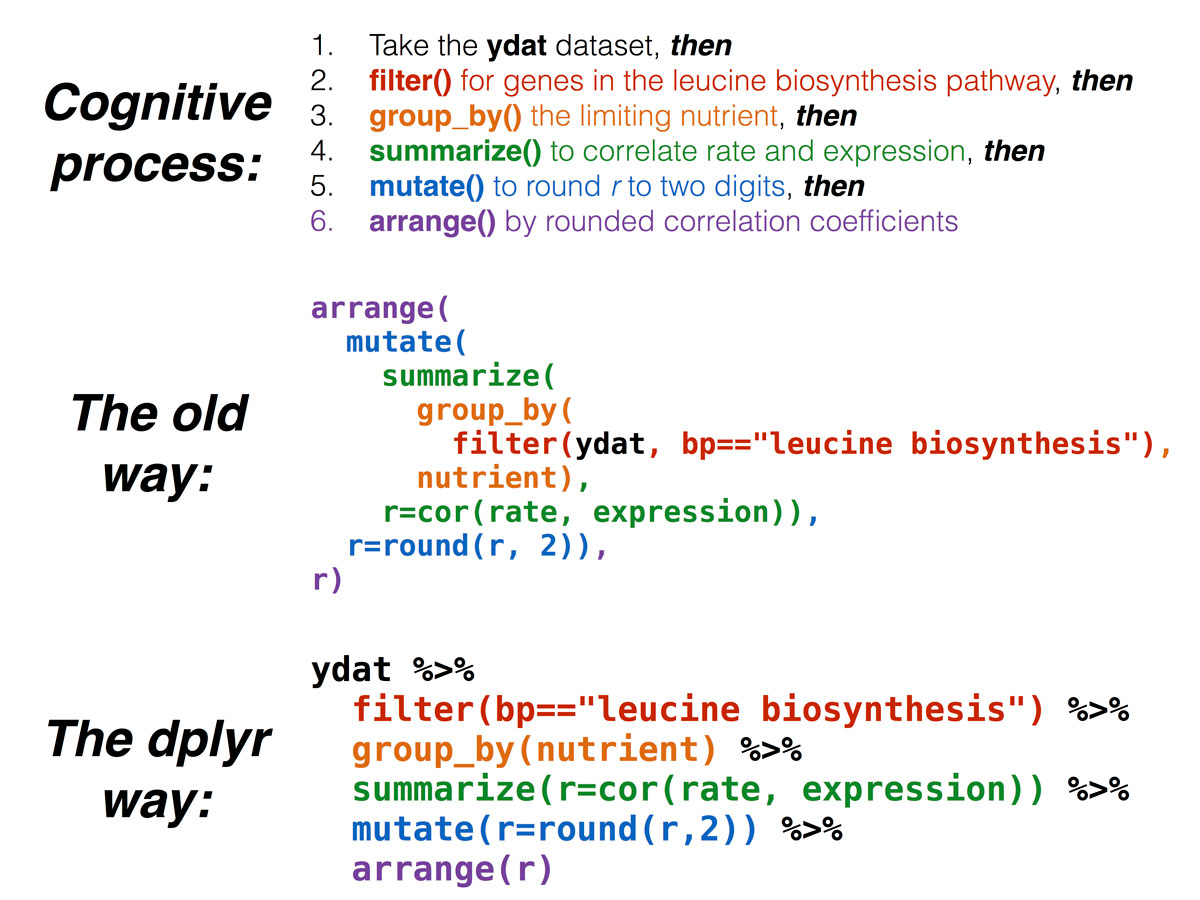
\includegraphics{nest_vs_pipe.jpg}

\hypertarget{switching-topics}{%
\subsubsection{Switching topics}\label{switching-topics}}

We'll now move into a couple topics that were not in previous problem
sets, but may be useful for a couple of the group projects.

\hypertarget{topic-7-finding-the-distance-between-points-coordinates}{%
\paragraph{Topic 7: Finding the distance between points
(coordinates)}\label{topic-7-finding-the-distance-between-points-coordinates}}

There is a package you can use to find the distance between points using
their latitude and longitude.

If you want to learn more about this package, you can follow
\href{https://cran.r-project.org/web/packages/geosphere/index.html}{this
link to the package documentation}.

The reference manual and a vignette are linked under documentation and
are good references for using the package.

\begin{Shaded}
\begin{Highlighting}[]
\CommentTok{\#call the package from your library}
\FunctionTok{library}\NormalTok{(geosphere)}
\CommentTok{\#read in a file with latitude and longitude for your points of interest}
\NormalTok{location }\OtherTok{\textless{}{-}} \FunctionTok{read.csv}\NormalTok{(}\StringTok{"location.csv"}\NormalTok{)}

\CommentTok{\#One method for determining the distance between two points is using the Haversine method. We\textquotesingle{}ll use the distm function in the geosphere package and then specify the Haversine method}

\CommentTok{\#first we need to get a dataframe that is just the latitude and longitude of our sites}
\CommentTok{\#for this example, those are columns 4 and 5}
\NormalTok{loc }\OtherTok{\textless{}{-}}\NormalTok{ location[}\DecValTok{4}\SpecialCharTok{:}\DecValTok{5}\NormalTok{]}

\CommentTok{\#if we want to do this with tidyverse, we would use:}
\NormalTok{loc2 }\OtherTok{\textless{}{-}}\NormalTok{ location }\SpecialCharTok{\%\textgreater{}\%} \FunctionTok{select}\NormalTok{(}\FunctionTok{c}\NormalTok{(better\_lat,better\_long))}

\NormalTok{distances}\OtherTok{\textless{}{-}}\FunctionTok{as.data.frame}\NormalTok{(}\FunctionTok{distm}\NormalTok{(loc,}\AttributeTok{fun=}\NormalTok{distHaversine))}

\NormalTok{distances}
\end{Highlighting}
\end{Shaded}

\begin{verbatim}
##           V1        V2         V3          V4          V5         V6         V7
## 1      0.000   660.877  8022.8087  7900.37420  7837.35339  8718.7374  8361.5898
## 2    660.877     0.000  7380.4758  7257.84625  7194.56792  8085.0650  7732.1484
## 3   8022.809  7380.476     0.0000   122.91365   187.02067   809.2943   664.6537
## 4   7900.374  7257.846   122.9136     0.00000    64.39771   920.4051   739.8633
## 5   7837.353  7194.568   187.0207    64.39771     0.00000   982.1989   789.1201
## 6   8718.737  8085.065   809.2943   920.40513   982.19893     0.0000   397.4869
## 7   8361.590  7732.148   664.6537   739.86327   789.12014   397.4869     0.0000
## 8   8149.464  8810.321 16060.1671 15939.88189 15878.87452 16697.3855 16318.8813
## 9   7291.742  7952.547 15201.8928 15081.53153 15020.46325 15841.0240 15463.1125
## 10  8737.038  9397.777 16630.6414 16510.64050 16449.86301 17262.2034 16882.2936
## 11 22834.952 23491.412 30821.7077 30700.55699 30638.80284 31473.3718 31097.4343
## 12 22534.567 23191.140 30520.4745 30399.34074 30337.60171 31171.7885 30795.7697
## 13 21559.856 22217.964 29529.7296 29408.93970 29347.49859 30173.6168 29795.7191
## 14 21328.766 21986.988 29297.2879 29176.52326 29115.10371 29940.6724 29562.6591
## 15 21273.830 21932.145 29241.0995 29120.36033 29058.96235 29883.9551 29505.8126
## 16  7776.517  7164.361  1151.1077  1133.27302  1136.71848  1214.4204   827.8534
##            V8         V9        V10       V11       V12        V13         V14
## 1   8149.4638  7291.7420  8737.0380 22834.952 22534.567 21559.8559 21328.76599
## 2   8810.3209  7952.5467  9397.7774 23491.412 23191.140 22217.9642 21986.98757
## 3  16060.1671 15201.8928 16630.6414 30821.708 30520.474 29529.7296 29297.28789
## 4  15939.8819 15081.5315 16510.6405 30700.557 30399.341 29408.9397 29176.52326
## 5  15878.8745 15020.4632 16449.8630 30638.803 30337.602 29347.4986 29115.10371
## 6  16697.3855 15841.0240 17262.2034 31473.372 31171.789 30173.6168 29940.67241
## 7  16318.8813 15463.1125 16882.2936 31097.434 30795.770 29795.7191 29562.65907
## 8      0.0000   859.6085   597.8743 14784.663 14482.670 13477.0371 13243.88217
## 9    859.6085     0.0000  1446.0147 15637.232 15335.340 14332.6579 14099.66611
## 10   597.8743  1446.0147     0.0000 14232.782 13930.623 12918.0293 12684.47188
## 11 14784.6632 15637.2324 14232.7823     0.000   302.263  1385.0338  1614.00022
## 12 14482.6698 15335.3397 13930.6233   302.263     0.000  1097.5474  1322.69540
## 13 13477.0371 14332.6579 12918.0293  1385.034  1097.547     0.0000   234.68694
## 14 13243.8822 14099.6661 12684.4719  1614.000  1322.695   234.6869     0.00000
## 15 13186.9641 14042.9311 12627.0568  1677.841  1387.056   295.8171    64.82476
## 16 15642.3681 14789.5076 16199.7238 30426.664 30124.736 29117.5697 28884.09397
##            V15        V16
## 1  21273.83022  7776.5168
## 2  21932.14533  7164.3609
## 3  29241.09954  1151.1077
## 4  29120.36033  1133.2730
## 5  29058.96235  1136.7185
## 6  29883.95506  1214.4204
## 7  29505.81263   827.8534
## 8  13186.96408 15642.3681
## 9  14042.93105 14789.5076
## 10 12627.05676 16199.7238
## 11  1677.84130 30426.6644
## 12  1387.05567 30124.7364
## 13   295.81706 29117.5697
## 14    64.82476 28884.0940
## 15     0.00000 28826.7493
## 16 28826.74929     0.0000
\end{verbatim}

The output of the \texttt{distm} function is a matrix of distances
between our points in meters. You'll have to reference the original list
to identify which bays each distance refers to.

In the \texttt{distm} command, we specified fun = distHaversine. There
are other options - distGeo or distCosine being two.

\hypertarget{topic-8-working-with-weather-data-or-other-messy-data}{%
\paragraph{Topic 8: working with weather data (or other messy
data)}\label{topic-8-working-with-weather-data-or-other-messy-data}}

Often when working with data, we will look to outside sources to
supplement our data. Sometimes, those outside sources will give us data
that is not easily worked with. In this example, we'll go through what
cleaning data may look like,

The data in this example were collected from the
\href{https://www.ncei.noaa.gov/cdo-web/}{NOAA Climate Data Online
page}.\\
This source gives weather data from multiple weather stations in the
area near a city (Augusta in this case). We may choose to only use some
weather stations depending on how complete these data are.

\begin{Shaded}
\begin{Highlighting}[]
\NormalTok{weather }\OtherTok{\textless{}{-}} \FunctionTok{read.csv}\NormalTok{(}\StringTok{"Augusta\_weather\_data.csv"}\NormalTok{)}

\CommentTok{\#what is the structure of the data}
\FunctionTok{str}\NormalTok{(weather)}
\end{Highlighting}
\end{Shaded}

\begin{verbatim}
## 'data.frame':    5934 obs. of  40 variables:
##  $ STATION  : chr  "US1SCAK0004" "US1SCAK0004" "US1SCAK0004" "US1SCAK0004" ...
##  $ NAME     : chr  "NORTH AUGUSTA 4.2 NE, SC US" "NORTH AUGUSTA 4.2 NE, SC US" "NORTH AUGUSTA 4.2 NE, SC US" "NORTH AUGUSTA 4.2 NE, SC US" ...
##  $ LATITUDE : num  33.6 33.6 33.6 33.6 33.6 ...
##  $ LONGITUDE: num  -81.9 -81.9 -81.9 -81.9 -81.9 ...
##  $ ELEVATION: num  74.7 74.7 74.7 74.7 74.7 74.7 74.7 74.7 74.7 74.7 ...
##  $ DATE     : chr  "1/4/2009" "1/7/2009" "1/11/2009" "1/18/2009" ...
##  $ AWND     : num  NA NA NA NA NA NA NA NA NA NA ...
##  $ DAPR     : int  NA NA NA NA NA NA NA NA NA NA ...
##  $ FMTM     : int  NA NA NA NA NA NA NA NA NA NA ...
##  $ MDPR     : num  NA NA NA NA NA NA NA NA NA NA ...
##  $ PGTM     : int  NA NA NA NA NA NA NA NA NA NA ...
##  $ PRCP     : num  0.12 0.39 0.45 0.29 0.04 0.27 0.01 0.13 0.12 0.08 ...
##  $ SNOW     : num  NA NA NA NA 0 NA NA NA NA NA ...
##  $ SNWD     : num  NA NA NA NA NA NA NA NA NA NA ...
##  $ TAVG     : logi  NA NA NA NA NA NA ...
##  $ TMAX     : int  NA NA NA NA NA NA NA NA NA NA ...
##  $ TMIN     : int  NA NA NA NA NA NA NA NA NA NA ...
##  $ TOBS     : logi  NA NA NA NA NA NA ...
##  $ WDF2     : int  NA NA NA NA NA NA NA NA NA NA ...
##  $ WDF5     : int  NA NA NA NA NA NA NA NA NA NA ...
##  $ WSF2     : num  NA NA NA NA NA NA NA NA NA NA ...
##  $ WSF5     : num  NA NA NA NA NA NA NA NA NA NA ...
##  $ WT01     : int  NA NA NA NA NA NA NA NA NA NA ...
##  $ WT02     : int  NA NA NA NA NA NA NA NA NA NA ...
##  $ WT03     : int  NA NA NA NA NA NA NA NA NA NA ...
##  $ WT04     : logi  NA NA NA NA NA NA ...
##  $ WT05     : int  NA NA NA NA NA NA NA NA NA NA ...
##  $ WT06     : logi  NA NA NA NA NA NA ...
##  $ WT07     : int  NA NA NA NA NA NA NA NA NA NA ...
##  $ WT08     : int  NA NA NA NA NA NA NA NA NA NA ...
##  $ WT09     : int  NA NA NA NA NA NA NA NA NA NA ...
##  $ WT11     : int  NA NA NA NA NA NA NA NA NA NA ...
##  $ WT13     : int  NA NA NA NA NA NA NA NA NA NA ...
##  $ WT14     : int  NA NA NA NA NA NA NA NA NA NA ...
##  $ WT16     : int  NA NA NA NA NA NA NA NA NA NA ...
##  $ WT17     : int  NA NA NA NA NA NA NA NA NA NA ...
##  $ WT18     : int  NA NA NA NA NA NA NA NA NA NA ...
##  $ WT19     : int  NA NA NA NA NA NA NA NA NA NA ...
##  $ WT21     : int  NA NA NA NA NA NA NA NA NA NA ...
##  $ WT22     : int  NA NA NA NA NA NA NA NA NA NA ...
\end{verbatim}

\begin{Shaded}
\begin{Highlighting}[]
\CommentTok{\#how many weather stations are there?}
\FunctionTok{length}\NormalTok{(}\FunctionTok{unique}\NormalTok{(weather}\SpecialCharTok{$}\NormalTok{STATION))}
\end{Highlighting}
\end{Shaded}

\begin{verbatim}
## [1] 14
\end{verbatim}

\begin{Shaded}
\begin{Highlighting}[]
\CommentTok{\#let\textquotesingle{}s rename some of these column names}
\NormalTok{weather }\OtherTok{\textless{}{-}}\NormalTok{ weather }\SpecialCharTok{\%\textgreater{}\%} \FunctionTok{rename}\NormalTok{(}\AttributeTok{precipitation =}\NormalTok{ PRCP,}
      \AttributeTok{max\_temp =}\NormalTok{ TMAX,}
      \AttributeTok{min\_temp =}\NormalTok{ TMIN,}
      \AttributeTok{average\_temp =}\NormalTok{ TAVG)}

\CommentTok{\#let\textquotesingle{}s look at which of the weather stations has the most observations each of these weather variables}
\CommentTok{\# !is.na filters out the NA values and n() counts the number of rows (non{-}NA observations)}

\NormalTok{weather }\SpecialCharTok{\%\textgreater{}\%} \FunctionTok{filter}\NormalTok{(}\SpecialCharTok{!}\FunctionTok{is.na}\NormalTok{(precipitation)) }\SpecialCharTok{\%\textgreater{}\%}
  \FunctionTok{group\_by}\NormalTok{(STATION) }\SpecialCharTok{\%\textgreater{}\%}
  \FunctionTok{summarize}\NormalTok{(}\AttributeTok{precip\_obs =} \FunctionTok{n}\NormalTok{())}
\end{Highlighting}
\end{Shaded}

\begin{verbatim}
## # A tibble: 14 x 2
##    STATION     precip_obs
##    <chr>            <int>
##  1 US1GACU0001        158
##  2 US1GACU0002        433
##  3 US1GACU0003        269
##  4 US1GACU0004         25
##  5 US1GARC0001        124
##  6 US1GARC0002        720
##  7 US1SCAK0004        153
##  8 US1SCAK0006         13
##  9 US1SCAK0010        712
## 10 US1SCAK0013        721
## 11 US1SCAK0017        621
## 12 US1SCAK0019        323
## 13 USW00003820        790
## 14 USW00013837        789
\end{verbatim}

\begin{Shaded}
\begin{Highlighting}[]
\NormalTok{weather }\SpecialCharTok{\%\textgreater{}\%} \FunctionTok{filter}\NormalTok{(}\SpecialCharTok{!}\FunctionTok{is.na}\NormalTok{(max\_temp)) }\SpecialCharTok{\%\textgreater{}\%}
  \FunctionTok{group\_by}\NormalTok{(STATION) }\SpecialCharTok{\%\textgreater{}\%}
  \FunctionTok{summarize}\NormalTok{(}\AttributeTok{precip\_obs =} \FunctionTok{n}\NormalTok{())}
\end{Highlighting}
\end{Shaded}

\begin{verbatim}
## # A tibble: 2 x 2
##   STATION     precip_obs
##   <chr>            <int>
## 1 USW00003820        790
## 2 USW00013837        787
\end{verbatim}

There are two weather stations, USW00003820 and USW00013837, that have
more complete data than the rest. We'll filter our data to just those
weather stations.

Now we'll summarize the weather data and look at precipitation and
temperature changes over time.

\begin{Shaded}
\begin{Highlighting}[]
\CommentTok{\#first, let\textquotesingle{}s make sure our date is in date format}
\NormalTok{weather}\SpecialCharTok{$}\NormalTok{DATE }\OtherTok{\textless{}{-}} \FunctionTok{mdy}\NormalTok{(weather}\SpecialCharTok{$}\NormalTok{DATE)}

\CommentTok{\#filter the data and summarize precipitation and max temperature data}
\NormalTok{weather\_summary }\OtherTok{\textless{}{-}}\NormalTok{ weather }\SpecialCharTok{\%\textgreater{}\%} \FunctionTok{filter}\NormalTok{(STATION}\SpecialCharTok{==}\StringTok{"USW00003820"}\SpecialCharTok{|}\NormalTok{STATION}\SpecialCharTok{==}\StringTok{"USW00013837"}\NormalTok{) }\SpecialCharTok{\%\textgreater{}\%}
  \FunctionTok{group\_by}\NormalTok{(DATE) }\SpecialCharTok{\%\textgreater{}\%}
  \FunctionTok{summarize}\NormalTok{(}\AttributeTok{mean\_precip =} \FunctionTok{mean}\NormalTok{(precipitation),}
            \AttributeTok{mean\_maxT =} \FunctionTok{mean}\NormalTok{(max\_temp))}

\CommentTok{\#let\textquotesingle{}s look at precipitation over time}
\FunctionTok{ggplot}\NormalTok{(weather\_summary,}\FunctionTok{aes}\NormalTok{(}\AttributeTok{x=}\NormalTok{DATE,}\AttributeTok{y=}\NormalTok{mean\_precip)) }\SpecialCharTok{+}
  \FunctionTok{geom\_point}\NormalTok{() }\SpecialCharTok{+}
  \FunctionTok{geom\_line}\NormalTok{() }\SpecialCharTok{+}
  \FunctionTok{theme\_classic}\NormalTok{()}
\end{Highlighting}
\end{Shaded}

\includegraphics{tidy_cheatsheet_for_group_project_files/figure-latex/unnamed-chunk-22-1.pdf}

\begin{Shaded}
\begin{Highlighting}[]
\CommentTok{\#that\textquotesingle{}s hard to interpret. Maybe it would be easier to look at with summaries for each month}
\CommentTok{\#first we\textquotesingle{}ll need a column with the month and year and then use that to group by and summarize like we did before}
\NormalTok{weather\_summary2 }\OtherTok{\textless{}{-}}\NormalTok{ weather }\SpecialCharTok{\%\textgreater{}\%} 
  \FunctionTok{mutate}\NormalTok{(}\AttributeTok{month\_year =} \FunctionTok{format}\NormalTok{(DATE,}\StringTok{"\%Y{-}\%m"}\NormalTok{)) }\SpecialCharTok{\%\textgreater{}\%}
  \FunctionTok{group\_by}\NormalTok{(month\_year) }\SpecialCharTok{\%\textgreater{}\%}
  \FunctionTok{summarize}\NormalTok{(}\AttributeTok{total\_precip =} \FunctionTok{sum}\NormalTok{(precipitation,}\AttributeTok{na.rm=}\NormalTok{T),}
            \AttributeTok{mean\_maxT =} \FunctionTok{mean}\NormalTok{(max\_temp,}\AttributeTok{na.rm=}\NormalTok{T))}

\FunctionTok{ggplot}\NormalTok{(weather\_summary2,}\FunctionTok{aes}\NormalTok{(}\AttributeTok{x=}\NormalTok{month\_year,}\AttributeTok{y=}\NormalTok{total\_precip)) }\SpecialCharTok{+}
  \FunctionTok{geom\_point}\NormalTok{() }\SpecialCharTok{+}
  \FunctionTok{theme\_classic}\NormalTok{()}
\end{Highlighting}
\end{Shaded}

\includegraphics{tidy_cheatsheet_for_group_project_files/figure-latex/unnamed-chunk-22-2.pdf}

\begin{Shaded}
\begin{Highlighting}[]
\CommentTok{\#it\textquotesingle{}s hard to read the x{-}axis, so we can use another line in our ggplot code to rotate the text}
\FunctionTok{ggplot}\NormalTok{(weather\_summary2,}\FunctionTok{aes}\NormalTok{(}\AttributeTok{x=}\NormalTok{month\_year,}\AttributeTok{y=}\NormalTok{total\_precip)) }\SpecialCharTok{+}
  \FunctionTok{geom\_point}\NormalTok{() }\SpecialCharTok{+}
  \FunctionTok{theme\_classic}\NormalTok{() }\SpecialCharTok{+}
  \FunctionTok{theme}\NormalTok{(}\AttributeTok{axis.text.x =} \FunctionTok{element\_text}\NormalTok{(}\AttributeTok{angle =} \DecValTok{90}\NormalTok{, }\AttributeTok{vjust =} \FloatTok{0.5}\NormalTok{, }\AttributeTok{hjust=}\DecValTok{1}\NormalTok{))}
\end{Highlighting}
\end{Shaded}

\includegraphics{tidy_cheatsheet_for_group_project_files/figure-latex/unnamed-chunk-22-3.pdf}

\begin{Shaded}
\begin{Highlighting}[]
\CommentTok{\#we can use the same code but replace total\_precip with mean\_maxT to look at average temperature}
\FunctionTok{ggplot}\NormalTok{(weather\_summary2,}\FunctionTok{aes}\NormalTok{(}\AttributeTok{x=}\NormalTok{month\_year,}\AttributeTok{y=}\NormalTok{mean\_maxT)) }\SpecialCharTok{+}
  \FunctionTok{geom\_point}\NormalTok{() }\SpecialCharTok{+}
  \FunctionTok{theme\_classic}\NormalTok{() }\SpecialCharTok{+}
  \FunctionTok{theme}\NormalTok{(}\AttributeTok{axis.text.x =} \FunctionTok{element\_text}\NormalTok{(}\AttributeTok{angle =} \DecValTok{90}\NormalTok{, }\AttributeTok{vjust =} \FloatTok{0.5}\NormalTok{, }\AttributeTok{hjust=}\DecValTok{1}\NormalTok{))}
\end{Highlighting}
\end{Shaded}

\includegraphics{tidy_cheatsheet_for_group_project_files/figure-latex/unnamed-chunk-22-4.pdf}

\textbf{And that's the end of the cheat sheet!} This cheat sheet is the
product of years of practice with R and isn't something that you should
expect to pick up immediately, but hopefully it's helpful as a reference

\end{document}
